\section{Security in the pipeline}
Security in the pipeline is the process of implementing different measures and controls to protect the code that is being sent through the pipeline from various security threats. The pipeline commonly consists of multiple phases like code development, testing, and deployment, all of which may be susceptible to various security threats, like unauthorized access, data breaches, malware, and denial-of-service attacks. Security in the pipeline is crucial to secure the integrity and confidentiality of software applications and data.
Below are tools that can be used for security in the pipeline and for a more in-depth explanation of the different tools, see chapter \ref{chap:Tools}. 

\subsection{Code Scanning}
\label{Code Scanning}
According to Microsoft's best practices for secure \acrshort{sdlc} \cite{microsoftSDLCpractices}, a SAST tool should be included in the pipeline. A SAST tool can be for example code scanning. Code scanning is a security measure where code is analyzed with the help of a tool to find security vulnerabilities and coding errors. Code scanning serves as a preventive measure against developers introducing new issues. In Figure \ref{fig: Pipeline with implemented SAST scan}, the \acrshort{sast} scan is set to be in GitHub. By doing this scan there, it is done at the earliest stage possible, before the code is moved forward in the pipeline, eliminating vulnerabilities as soon as possible.

 \vspace{2mm}
\begin{figure}[H]
    \centering
    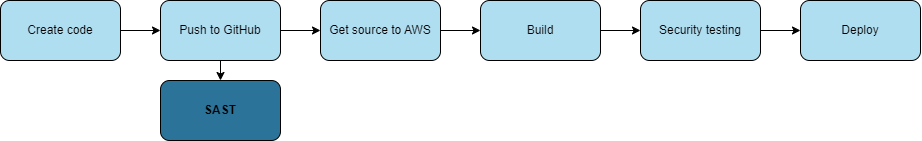
\includegraphics[width=0.8\columnwidth]{Images/pipeline2.png}
    \caption{Pipeline with implemented SAST scan}
    \label{fig: Pipeline with implemented SAST scan}
\end{figure}

\subsection{Scan Dependencies and Open Source Libraries}
\label{Scan Dependencies and Open Source Libraries}
Dependencies can be divided into two parts: direct and transitive. A direct dependency is directly referenced software component in an application. A transitive one is a functional software component necessary for an application's direct \gls{dependency}. These \gls{dependency} may have their own set of direct and indirect \gls{dependency}, resulting in a recursive tree of transitive \gls{dependency} affecting the application. This essentially means that the \gls{dependency} used in the code may be linked to numerous additional dependents, creating a large supply chain. To secure these supply chains, in addition to vulnerability scanning, the company can create a clear policy for evaluating and managing \gls{dependency}, including criteria for selecting secure and trustworthy libraries and frameworks. They should also limit the use of unnecessary or outdated \gls{dependency}, as these can increase the attack surface and create unnecessary risk. \cite{googledependency}
\\~\\
All dependencies, open-source libraries, and third-party \gls{artifact}s that have been utilized should be validated. To validate a file's integrity, compare the hash of an artifact to the hash value generated by the artifact provider. This comparison helps in detecting any unauthorized alterations, tampering, or corruption of dependencies that may occur as a result of a man-in-the-middle attack or a compromise of the artifact repository. If any third-party software was implemented in the application it's important to conduct an \acrshort{sca} scan using suitable tools to identify whether any vulnerable open-source software was used. \cite{bestpracticeSupplyChain}
\\~\\
The \acrshort{sca} is placed in combination with the \acrshort{sast} tool in Figure \ref{fig: Pipeline with implemented SCA scan}. Similarly to \acrshort{sast}, it is done in GitHub to patch the vulnerable \gls{dependency} early in the implementation phase.

\vspace{2mm}
\begin{figure}[H]
    \centering
    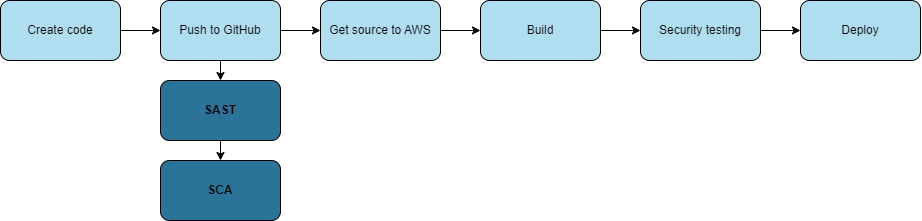
\includegraphics[width=0.8\columnwidth]{Images/pipeline3.png}
    \caption{Pipeline with implemented SCA scan}
    \label{fig: Pipeline with implemented SCA scan}
\end{figure}

\subsection{Secret Scanning}
To prevent or identify accidental exposure of \say{secrets}, like access tokens, SSH keys, or other credentials, one should execute a secret scanning on the repository the source code is stored. Such secrets can give unwanted access to accounts, software, or cloud providers, among other things. With access to for example cloud credentials, a threat actor could, among other harmful attacks, scale up the use of various costly resources, costing a company much more than what they have budgeted for \cite{GitGuardianexploitexample}. According to GitGuardian's early report on secret leaks \cite{GitGuardiansecretsprawl}, they detected 10 million secrets leaked in 2022, which is an increase of 67\% from 2021. The same report showed 1 in 10 GitHub authors had exposed a secret in their repository. This shows an increasing issue with secret leaks. Secret scanning tools can be used to find these vulnerabilities, and alert developers to potential security risks. \cite{GithubSecretScanning} 
\\~\\
In Figure \ref{fig: Pipeline with implemented secret scan}, secret scanning is recommended to be done together with \acrshort{sast} and \acrshort{sca} for the same reason, explained in \ref{Code Scanning} and \ref{Scan Dependencies and Open Source Libraries}.

\vspace{2mm}
\begin{figure}[H]
    \centering
    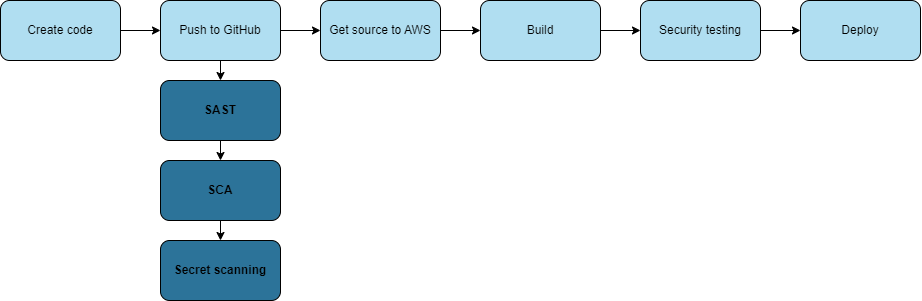
\includegraphics[width=0.8\columnwidth]{Images/pipeline4.png}
    \caption{Pipeline with implemented secret scan}
    \label{fig: Pipeline with implemented secret scan}
\end{figure}

\subsection{Dynamic scanning}
In software best practices, it is recommended to run multiple tests and scans to identify bugs and errors - where one of these tests is \acrlong{dast} (\acrshort{dast}) \cite{bestpracticeSupplyChain}. This scanning method tries to penetrate the application, attempting to identify vulnerabilities and weaknesses in it. One can implement a tool specialized for DAST scans, such as OWASP Zap, which can identify security risks like \gls{Cross-site scripting}, \gls{SQL-injection} or path traversal.\cite{dynamictesting}


\subsubsection{The Limitations of DAST Tools}
Even though \acrshort{dast} can be used to identify potential vulnerabilities, certain types of threats may go undetected. For this reason, the company should engage a red team, which is a group of experts capable of performing penetration testing. A penetration test will provide a more realistic test, as it simulates a real-world attack, detects more complex vulnerabilities, and provide a more comprehensive view of an application's security posture. A pen test can also function as a validation of the \acrshort{dast} scan, as it can help determine if the vulnerability can be exploited and the potential impact of the vulnerability. \cite{dastpentesting}
\\~\\
In Figure \ref{fig: Pipeline with implemented DAST scan and pentesting} the \acrshort{dast} scan and penetration test is placed later in the pipeline because these tests are executed on a running application. Therefore, the tests can not be done any earlier, yet they should be done before the application is deployed.
\vspace{2mm}
\begin{figure}[H]
    \centering
    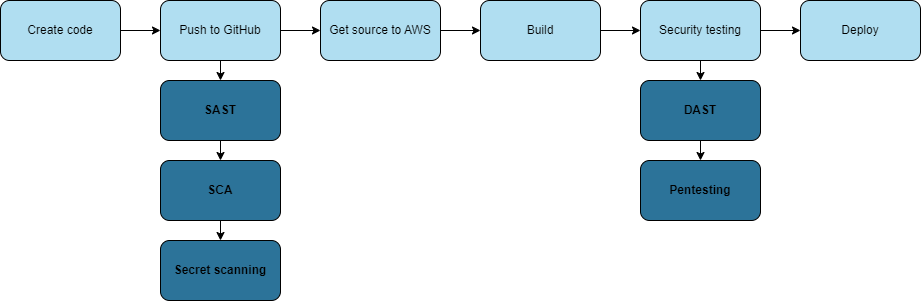
\includegraphics[width=0.8\columnwidth]{Images/pipeline5.png}
    \caption{Pipeline with implemented DAST scan and pentesting}
    \label{fig: Pipeline with implemented DAST scan and pentesting}
\end{figure}